\documentclass[a4paper,12pt]{Latex/Classes/PhDthesisPSnPDF}
\usepackage[utf8]{inputenc}
\usepackage{amsthm}
\usepackage{graphicx}

% \usepackage[spanish]{babel}
% \input{body/preamble/preamble.Rnw}
% This file contains macros that can be called up from connected TeX files
% It helps to summarise repeated code, e.g. figure insertion (see below).

%%%%%%%%%%%%%%%%%%%%%%%%%%%%%%%%%%%%%%%%%%%%%%
%            Colores de la UNAM              %
%%%%%%%%%%%%%%%%%%%%%%%%%%%%%%%%%%%%%%%%%%%%%%
%Azul Pantone 541  -->(0,63,119) RGB
\definecolor{Azul}{RGB}{128,0,0}

%Oro Pantone 460  -->(234,221,150) RGB
\definecolor{Oro}{RGB}{234,221,150}


%%%%%%%%%%%%%%%%%%%%%%%%%%%%%%%%%%%%%%%%%%%%%%
%            Comandos para líneas            %
%%%%%%%%%%%%%%%%%%%%%%%%%%%%%%%%%%%%%%%%%%%%%%
%Se define un comando \colorvrule para hacer líneas verticales de color con 3 argumentos: color, ancho, alto
\newcommand{\colorvrule}[3]{
\begingroup\color{#1}\vrule width#2 height#3
\endgroup}

%Se define un comando \colorhrule para hacer líneas horizontales de color con 2 argumentos: color, ancho
\newcommand{\colorhrule}[2]{
\begingroup\color{#1}\hrule height#2
\endgroup}

%%%%%%%%%%%%%%%%%%%%%%%%%%%%%%%%%%%%%%%%%%%%%%
%          Comando para derivadas            %
%%%%%%%%%%%%%%%%%%%%%%%%%%%%%%%%%%%%%%%%%%%%%%
\newcommand{\derivada}[3][]{\ensuremath{\dfrac{\mbox{d}^{#1}#2}{\mbox{d}#3^{#1}}}} 
%primer argumento(opcional): orden de la derivada
%segundo argumento: función a derivar
%tercer argumento: variable respecto a la que se deriva


%%%%%%%%%%%%%%%%%%%%%%%%%%%%%%%%%%%%%%%%%%%%%%
%       Comando para la exponencial          %
%%%%%%%%%%%%%%%%%%%%%%%%%%%%%%%%%%%%%%%%%%%%%%
\newcommand{\e}[1][]{\ensuremath{\mbox{e}^{#1}}}
%primer argumento(opcional): exponente de la exponencial




% insert a centered figure with caption and description
% parameters 1:filename, 2:title, 3:description and label
\newcommand{\figuremacro}[3]{
	\begin{figure}[htbp]
		\centering
		\includegraphics[width=1\textwidth]{#1}
		\caption[#2]{\textbf{#2} - #3}
		\label{condicion}
	\end{figure}
}

% insert a centered figure with caption and description AND WIDTH
% parameters 1:filename, 2:title, 3:description and label, 4: textwidth
% textwidth 1 means as text, 0.5 means half the width of the text
\newcommand{\figuremacroW}[4]{
	\begin{figure}[htbp]
		\centering
		\includegraphics[width=#4\textwidth]{#1}
		\caption[#2]{\textbf{#2} - #3}
		\label{#1}
	\end{figure}
}

% inserts a figure with wrapped around text; only suitable for NARROW figs
% o is for outside on a double paged document; others: l, r, i(inside)
% text and figure will each be half of the document width
% note: long captions often crash with adjacent content; take care
% in general: above 2 macro produce more reliable layout
\newcommand{\figuremacroN}[3]{
	\begin{wrapfigure}{o}{0.5\textwidth}
		\centering
		\includegraphics[width=0.48\textwidth]{#1}
		\caption[#2]{{\small\textbf{#2} - #3}}
		\label{#1}
	\end{wrapfigure}
}

% predefined commands by Harish
\newcommand{\PdfPsText}[2]{
  \ifpdf
     #1
  \else
     #2
  \fi
}

\newcommand{\IncludeGraphicsH}[3]{
  \PdfPsText{\includegraphics[height=#2]{#1}}{\includegraphics[bb = #3, height=#2]{#1}}
}

\newcommand{\IncludeGraphicsW}[3]{
  \PdfPsText{\includegraphics[width=#2]{#1}}{\includegraphics[bb = #3, width=#2]{#1}}
}

\newcommand{\InsertFig}[3]{
  \begin{figure}[!htbp]
    \begin{center}
      \leavevmode
      #1
      \caption{#2}
      \label{#3}
    \end{center}
  \end{figure}
}







%%% Local Variables:
%%% mode: latex
%%% TeX-master: "~/Documents/LaTeX/CUEDThesisPSnPDF/thesis"
%%% End:
 
\newtheorem{teorema}{Teorema}
\newtheorem{definicion}{Definición}
% \showboxdepth=5
% \showboxbreadth=5
%%%%%%%%%%%%%%%%%%%%%%%%%%%%%%%%%%%%%%%%%%%%%%%%%%%%%%%%%%%%%%%%%%%%%%%%%%%%%%%%
%                                   DATOS                                      %
%%%%%%%%%%%%%%%%%%%%%%%%%%%%%%%%%%%%%%%%%%%%%%%%%%%%%%%%%%%%%%%%%%%%%%%%%%%%%%%%
\title{Evaluación de la Eficacia de una estrategia de trading basada en Modelo Lineal Generalizado}
\author{Rodrigo Alejandro Serrano Morales} 
\facultad{Facultad de Ciencias Económicas y Sociales\\
Escuela de Estadística y Ciencias Actuariales}                % Nombre de la facultad/escuela
\escudofacultad{images/faces} % Aquí ponen la ruta y nombre del escudo de su facultad, actualmente, la carpeta Latex/Classes/Escudos cuenta con los siguientes escudos:
% "fi_azul" Facultad de ingenieria en color azul
% "fi_negro" Facultad de ingenieria en color negro
% "fc_azul" Facultad de ciencias en color azul
% "fc_negro" Facultad de ciencias en color negro
% Se agradecen sus aportaciones de escudos a jebus.velazquez@gmail.com

\degree{Licenciado en Ciencias Actuariales}        % Carrera
\director{Prof. Jonattan Ramos \& Prof. Eloy Eligon}               % Director de tesis
\degreedate{Marzo 2019}                           % Año de la fecha del examen
\lugar{Caracas}                        % Lugar

%\portadafalse                              % Portada en NEGRO, descomentar y comentar la línea siguiente si se quiere utilizar
\portadatrue                                % Portada en COLOR



%% Opciones del posgrado (descomentar si las necesitan)
	%\posgradotrue                                                    
	%\programa{programa de maestría y doctorado en ingeniería}
	%\campo{Ingeniería Eléctrica - Control}
	%% En caso de que haya comité tutor
	%\comitetrue
	%\ctutoruno{Dr. Emmet L. Brown}
	%\ctutordos{Dr. El Doctor}
%% Datos del jurado                             
	%\presidente{Dr. 1}
	%\secretario{Dr. 2}
	%\vocal{Dr. 3}
	%\supuno{Dr. 4}
	%\supdos{Dr. 5}
	%\institucion{el Instituto de Ingeniería, UNAM}

\keywords{tesis,autor,tutor,etc}            % Palablas clave para los metadatos del PDF
\subject{tema_1,tema_2}                     % Tema para metadatos del PDF  

%%%%%%%%%%%%%%%%%%%%%%%%%%%%%%%%%%%%%%%%%%%%%%%%%%%%%
%                   PORTADA                         %
%%%%%%%%%%%%%%%%%%%%%%%%%%%%%%%%%%%%%%%%%%%%%%%%%%%%%
\usepackage{Sweave}
\begin{document}
\Sconcordance{concordance:main.tex:main.Rnw:%
1 64 1 1 0 14 1}
\Sconcordance{concordance:main.tex:./body/introduccion/introduccion.Rnw:ofs 80:%
1 11 1}
\Sconcordance{concordance:main.tex:./body/chapter1/chapter1.Rnw:ofs 92:%
1 43 1}
\Sconcordance{concordance:main.tex:./body/chapter2/chapter2.Rnw:ofs 136:%
1 255 1 1 18 1 2 17 1}
\Sconcordance{concordance:main.tex:./body/chapter3/chapter3.Rnw:ofs 411:%
1 95 1 1 64 3 1 2 2 32 1}
\Sconcordance{concordance:main.tex:./body/chapter4/chapter4.Rnw:ofs 545:%
1 15 1 1 14 3 1 2 2 13 1 1 8 1 3 7 1 1 8 1 2 4 1 1 74 2 1 1 3 1 2 8 1 1 %
3 1 2 8 1 1 3 1 2 8 1 1 12 5 1 1 9 1 2 12 1 1 14 1 2 9 1 1 3 1 2 13 1 1 %
7 1 2 4 1 1 7 3 1 1 7 1 2 22 1 1 3 9 0 1 2 1 1 1 32 1 2 8 0 1 1 7 0 1 2 %
9 0 1 1 10 0 1 2 12 1 1 7 12 0 1 2 3 1 1 6 12 0 1 2 3 1 1 6 12 0 1 2 4 %
1 1 6 12 0 1 2 3 1 1 6 12 0 1 2 4 1 1 6 12 0 1 2 7 1 1 37 2 1 1 2 15 0 %
1 2 3 1 1 26 5 1 1 9 1 2 4 1 1 24 3 1 1 9 1 2 15 1 1 17 2 1 1 2 14 0 1 %
2 3 1 1 27 2 1 1 2 11 0 1 2 2 1}
\Sconcordance{concordance:main.tex:./body/conclusion/conclusion.Rnw:ofs 976:%
1 7 1 1 20 3 1 1 6 1 2 15 1}
\Sconcordance{concordance:main.tex:./body/anexos/anexos.Rnw:ofs 1005:%
1 9 1 1 2 12 0 1 2 3 1 1 2 12 0 1 2 2 1 1 2 12 0 1 2 5 1 1 2 12 0 1 2 3 %
1 1 2 12 0 1 2 2 1 1 2 12 0 1 2 6 1 1 2 12 0 1 2 3 1 1 2 12 0 1 2 3 1 1 %
2 12 0 1 2 5 1 1 2 12 0 1 2 3 1 1 2 12 0 1 2 2 1 1 2 12 0 1 2 6 1 1 2 %
12 0 1 2 3 1 1 2 12 0 1 2 2 1 1 2 12 0 1 2 5 1 1 2 12 0 1 2 3 1 1 2 12 %
0 1 2 2 1 1 2 12 0 1 2 6 1 1 2 12 0 1 2 4 1 1 2 12 0 1 2 2 1 1 2 12 0 1 %
2 5 1 1 2 12 0 1 2 3 1 1 2 12 0 1 2 2 1 1 2 12 0 1 2 1 1}
\Sconcordance{concordance:main.tex:./body/bibliografia/bibliografia.Rnw:ofs 1432:%
1 37 1}
\Sconcordance{concordance:main.tex:main.Rnw:ofs 1470:%
88 1 1}


\maketitle									% Se redefinió este comando en el archivo de la clase para generar automáticamente la portada a partir de los datos

\newpage\renewcommand{\thepage}{\arabic{page}}\setcounter{page}{1} 

% !TeX root = ./main.Rnw
%\SweaveUTF8

\begin{dedication}
Dedicado a mis padres y a mi hermana, por ser los pilares de mi vida y ser mi motivo de haber cumplido esta meta.
\end{dedication}
% !TeX root = ./main.Rnw
%\SweaveUTF8
\newpage
\chapter*{Agradecimientos}

Agradecimientos




  \begin{flushright}
  \textbf{Gracias}
  \end{flushright}

\tableofcontents
\listoffigures
\listoftables


% !TeX root = ./main.Rnw
%\SweaveUTF8

\chapter*{Introducción}
\addcontentsline{toc}{chapter}{Introduccion}

Las economías de países latinoamericanos son reconocidas históricamente por depender en gran magnitud del comercio de sus materias primas, lo cual hace que el comercio con dichos commodities resulte de gran impacto para el gasto fiscal y para la balanza de pagos, esto deja como consecuencia, la necesidad de los actores económicos de estudiar el riesgo a profundidad para poder evitar resultados que reduzcan sus retornos positivos.\\ 

% !TeX root = ./main.Rnw
%\SweaveUTF8

\chapter{El Problema}

\section{Justificación}


\section{Planteamiento del Problema}


\section{Objetivo General}

Evaluar la eficacia de una estrategia de trading basada en técnicas de aprendizaje automático en diferentes instrumentos financieros

\section{Objetivos Específicos}

\begin{itemize}
\item Definir los parámetros de la estrategia, así como los indicadores técnicos a utilizar como variables predictoras
\item Utilizar Análisis de Componentes Principales como técnica de reducción de la dimensión de variables predictoras
\item Aplicar método de Regresión Logística con las componentes arrojadas por el ACP
\item Desarrollar la metodología Walkforward para tomar en cuenta el dinamismo del mercado en la estrategia
\item Evaluar la predicción del modelo como estrategia en los instrumentos seleccionados
\end{itemize}

% !TeX root = ./main.Rnw
%\SweaveUTF8

\chapter{Marco Teórico}

\section{Antecedentes}

\subsection{Trading de Cryptomonedas basado en Aprendizaje Automatico}

\subsection{Modelos predictivos para el mercado FOREX}

\subsection{Diseño e implementación de un sistema automatizado para operar en el mercado de divisas usando reglas de asociación}

\section{Bases Teóricas}


\subsection{Hipótesis del Mercado Eficiente}

La Hipótesis del Mercado eficiente fue desarrollada por Eugene Fama en los años 60, en la misma argumenta que los precios de los activos reflejan toda la información disponible, es decir que siempre son transados a un valor adecuado para su riesgo, haciendo imposible para los inversores obtener retornos más elevados que los del mercado en general. 

Fama sugiere tres suposiciones. Primero, el mercado eficiente requiere un gran número de competidores buscando maximizar ganancias. Segundo, la información que afecta al activo llega al mercado de manera aleatoria y cada anuncio es independiente de los demás. Tercero, todos los competirdores intentarán ajustar sus posiciones lo más rapido posible conocida la información del mercado. Existen tres variantes de la hipótesis:

$Eficiencia débil$, en esta variante, los precios del pasado no sirven para predecir el precio futuro, es decir cualquier movimiento del activo es determinado por información no contenida en la serie de precios. $Eficiencia media$, en esta forma se asume que los precios se ajustan instantáneamente a la información pública, por lo que rechaza cualquier tipo de arbitraje intentando aprovechar nueva información. $Eficiencia fuerte$, esta última forma de la hipótesis plantea que los precios reflejan tanto información pública como privada, por lo cual incluso obteniendo información no conocida por todos los competidores, no se pueden obtener retornos anormales a los de los mercados.

Aunque esta hipótesis es la piedra angular de la teoría financiera moderna, es controversial entre la comunidad financiera y dispustada frecuentemente. Gran parte de sus detractores argumentan que el precio del activo está influenciado por suposiciones cesgada de los individuos, formuladas por la manera en como estos responden ante nueva información. Algunas de las hipótesis que explican este razonamieto cesgado son: 

Los inversores interpretan la información de manera distinta, por lo que generarán diferentes valuaciones de un mismo activo, lo que sugiere que la reacción del inversor a la misma noticia será distinta. Day and Wangr (2002) argumentan que si los precios son continuamente influenciados por estas interpretaciones erróneas, los movimientos contrarios del precio pueden ser predecidos estudiando la data histórica. Sugieren también que mientras más extremo sea el movimiento incial, mayor será el ajuste de precio.

Los inversores se dejan influenciar por la tendencia del mercado, este comportamiento se ha visto a lo largo de la historia en casos de colapso del mercado como en la caída del mercado búrsatil en 1987 ó la burbuja del puntocom a finales de los 90. Froot (1992) muestra como estos comportamientos pueden resultar en ineficiencias del mercado.

Aglunos académicos como Hong y Stein's (1999) categorizan a los inversores en $Informados$ y $No informados$. Los inversores que tienen acceso a la información solo operan al obtener nueva información, mientras que los no informados operan basados en el pasado reciente del activo. A medida que la información es conocida por todos los competidores, se forma el fenómeno de reversión a la media.

Es evidente la postura que se asume en la presente investigación con respecto a la hipótesis de mercado eficiente. Además de los aspectos del comportamiento de los competires, se ha evidenciado en la historia, casos de inversores que han logrado vencer el mercado por largos períodos de tiempo, como Warren Buffet, lo cual por definición de la hipótesis es imposible. Por otro lado, Los avances técnologicos y la capacidad de procesamiento de las computadoras en la actualidad hacen pensar que cualquier anomalía presente en el mercado por muy pequeña que sea puede ser aprovechada por sofisticados softwares automatizados.

\subsection{Análisis Técnico}

Los inversionistas que rechazan la hipótesis del mercado eficiente buscan interpretar la situación del mercado, bien a través de noticias que afecten al activo o estudiando su movimiento intentando extrer patrones de conducta. A la primera técnica se le llama $Análisis Fundamental$ y el segundo $Análisis Técnico$. El Análisis Fundamental está mas asociado a estrategias de inversión pasivas a largo plazo aunque en la actualidad se han desarrollado algoritmos de compra y venta que buscan predecir la dirección del precio en función de noticas utilizando minería de texto.

El análisis técnico es aquel que busca patrones y tendencias de comportamiento en la cotización de los activos financieros, basándose en la serie de tiempo del activo, con esto intenta predecir el movimiento futuro mediante el uso de gráficos. Según J.J.Murphy (1999) existen tres fundamentos básicos en los que se basa el análisis técnico: Los movimientos del mercado lo descuentan  todo, los precios se mueven por tendencias y la historia se repite.

Murphy establece que cualquier efecto que posiblemente pueda afectar al precio se ve reflejado en la cotización del mismo. Por lo que un estudio del desplazamiento del activo en un período de tiempo sería suficiente para lograr predecir su movimiento. Esto quiere decir que el análisis técnico no es mas que una manera indirecta de estudiar los fundamentos del activo, suponiendo que la cotización del mismo resume toda la información que lo afecta. 

El análista técnico acepta la premisa de que los mercados tienen tendencias. Buscar tendencias en las primeras etapas de su desarrollo es la razón de toda la representación gráfica dentro del análisis, con el fin de que las transacciones vayan en dirección de esa tendencia. Por otro lado, la afirmación de que la historia se repite tiene que ver con el estudio de la psicología humana, la cual según murphy se repite. Ésta afirmación tiene también una estrecha relación en los ciclos económicos. 

\subsection{Introducción al aprendizaje automático}

Aprendizaje automático refiere a una rama de la Inteligencia Artificial, que busca crear algoritmos capaces de generalizar comportamientos y reconocer patrones a partir de un conjunto de datos. Supongamos que existe una variable respuesta $Y$ y distintos predictores $X_{1}, X_{2}, ..., X_{j}$. Se asume que existe una relación entre $Y$ y $X = X_{1}, X_{2}, ..., X_{j}$, la cual puede ser escrita de forma general como

$$ Y = f(X) + \epsilon $$

donde $f$ es una función desconocida de $X$ y $\epsilon$ es un término de error aleatorio, independiente de $X$ y de media 0. En esta formulación $f$ representa información sistemática que $X$ proporciona sobre $Y$.

En escencia, el aprendizaje automático refiere a un conjunto de enfoques para estimar $f$

\subsubsection{Métodos Paramétricos vs No Paramétricos}

La mayoría de los metodos de aprendizaje automático pueden ser caracterizados como paramétricos o no paramétricos. Los primeros, involucran un enfoque basado en dos pasos. Primero se asume que los datos toman una forma específica, una vez asumida la forma que debe tener la función $f$, el problema de la estimación se simplifica. al seleccionar el modelo se procede a ajustar el modelo en la data de entrenamiento. Este es el caso de los Modelos Lineales Generalizados como la Regresión Logística. La desventaja de este enfoque paramétrico es que el modelo escogido puede no ser apropiado a la verdadera forma de $f$, por lo que la estimación puede ser pobre.

Por otro lado los modelo No Paramétricos no asumen ninguna forma para $f$, en cambio, estos modelos buscan estimar $f$ acercandola lo mas posible a los datos observados. Esto les permite evadir el problema de ajustarse a alguna forma en específico. Sin embargo, al no reducir el problema a estimar unos parámetros sino uilizar los datos directamente, se necesita un gran numero de observaciones -muchas más que las necesarias por los métodos paramétricos- para obtener una estimación precisa. Además en general la iterpretación del modelo se hace más difícil con estos métodos y son propensos a caer en sobreoptimización

\subsubsection{Aprendizaje Supervisado vs No Supervisado}

Se le llama aprendizaje Supervisado, a los métodos en los cuales para cada observación de las variables predictoras $x_{i}$ existe un valor asociado a la variable respuesta $y_{i}$. Por lo que se ajusta un modelo que relacione la respuesta con los predictores, con el fin de predecir acertivamente respuestas futuras. Este es el caso de los modelos Lineales así como los métodos de boosting, SVM, GAM, etc. 

En contraste, lo métodos No Supervisados describen una situación más complicada, en donde para cada observación, se cuenta con variables predictoras, pero no existe ninguna variable respuesta. Lo que se busca en este tipo de modelos es buscar entender la relación entre las variables o entre las observaciones. Para esto se utilizan métodos de agrupación o cluster y métodos de reglas de asociasión. Los primeros intentan describir las agrupaciones subyacientes en los datos, como por ejemplo, el tipo de clientes dependiendo de su comportamiento de compra. Las reglas de asociasion buscan descrubrir patrones inehentes que describan el comportamiento de los datos u observaciones, por ejemplo, un grupo de clientes que compran un producto $r$ conjunto con otro producto $s$.

\subsubsection{Regresión vs Clasificasión}

Las variables pueden ser divididas entre cuantitativas ó cualitativas -también llamadas categóricas-. Las cuantitativas toman valores numericos mientras que las cualitativas son categorías o clases. Dependiendo del tipo de variable respuesta se realiza el enfoque del modelo. En el caso de que la variable respuesta sea cuantitavia se refiere a problemas de regresión, mientras que los que involucran una variable respuesta cualitativa, son referidos como problemas de clasificación.

\subsubsection{Compensasión entre sesgo y varianza}


\subsection{Regresión Logística}

Los modelos Lineales Generalizados asumen que exite una aproximada relación lineal entre la variable respuesta $Y$ y la variable predictora $X$. Matemáticamente se puede describir la relación como:

$$ Y \approx \beta_{0} + \beta_{1}X_{1} + ... + \beta_{j}X_{j} $$

En donde $X_{j}$ representa las variables predictoras y los coeficientes $\beta_{j}$ cuantifican la asociación entre la variable predictora $X_{j}$ y la variable respuesta $Y$. Por lo que se interpreta a $\beta_{j}$ como el efecto promedio que tiene en $Y$ un incremento de una unidad en $X_{j}$, bajo el supuesto de que todas las demás variables se mantienen constantes.

En problemas de clasificación, la variable predictora asume valores categóricos, por lo que al utilizar este enfoque se pueden obtener probabilidades fuera del intervalo [0, 1], haciendo imposible su interpretación. Esto concluye en que se deba utilizar una función, tal que permita la generación de valores entre [0, 1], en el caso de la regresión logística esta función es:

$$
p(X) = \frac{e^{\beta_{0} + \beta_{1}X_{1} + \beta_{2}X_{2} + ... + + \beta_{j}X_{j} }}{1 + e^{\beta_{0} + \beta_{1}X_{1} + \beta_{2}X_{2} + ... + + \beta_{j}X_{j} }}
$$

Despejando se obtiene

$$ \frac{p(X)}{1 - p(X)} = e^{\beta_{0} + \beta_{1}X_{1} + \beta_{2}X_{2} + ... + + \beta_{j}X_{j} } $$

El lado izquierdo de la ecuación puede tomar valores entre 0 e \infinity, lo cual indicaría muy bajas o muy altas probabilidades, aplicando logarítmo en ambos miembros de la ecuación se obtiene la función logit

$$ \log{\frac{p(X)}{1 - p(X)}} = \beta_{0} + \beta_{1}X_{1} + \beta_{2}X_{2} + ... + + \beta_{j}X_{j}  $$

Se observa que la función logit es lineal en $X$, por lo que incrementar una unidad de $X$ afecta el lado izquierdo de la ecuación en $\beta$. Sin embargo dado que la relación entre $p(X)$ y $X$ no es una linea recta, $\beta$ no corresponde a un cambio en $p(X)$ asosiado a una unidad de incremento en $X$. Se debe hacer la respectiva transformación para interpretar el coeficiente $\beta$ en relación a $Y$.

\subsubsection{Máxima Verosimilitud}

Los coeficientes $\beta$ son desconocidos, por lo que deben estimarse en la data de entrenamiento. Para esto se utiliza el metódo de $Máxima Verosimilitud$, el cual consiste en estimar los coeficientes para los cuales la probabilidad de prediccion para cada individuo, utilizando (formula arriba), corresponda lo más cercano posible al valor observado del individuo. Se define la función de verosimilitud como

$$ l(\beta) = \prod_{i=1}^{j}{P(x_{i} / \beta)} $$
  
Por conveniencia se  trabaja con el logarítmo, dado que esto transforma una operación de productos de probabilidades en una sumatoria, por lo que se obtiene

$$ l(\beta) = \sum_{i=1}^{N} \log{P(y_{i}/ x_{i}; \beta)} $$

Al codificar las clases en 0 y 1, la función de verosimilitud para la regresión logarítmica puede ser escrita como

$$ l(\beta) = \sum_{i=1}^{N}(y_{i}\beta^{T}x_{i} - \log{1 + e^{\beta^{T}x_{i}}}) $$

Para maximizar la función, se iguala la derivada a 0

$$ \frac{\partial l(\beta)}{\partial \beta} = \sum_{i=1}^{N}x_{i}(y_{i} - P(x_{i}; \beta)) = 0 $$

Para resolver la ecuación (n arriba) se utiliza un algoritmo de optimización llamado $Newton-Raphson$

\subsection{Análisis de Componentes Principales como método de reducción de variables}

Los modelos lineales tienen distintas ventajas en cuanto a interpretación y muchas veces son sorprendentemente competitivos en relación con los metodos no lineales. Exiten técnicas para relajar el supuesto de  que la relación entre la respuesta y los predictores es lineal, arrojando mejores predicciones e interpretabilidad. 

Una clase de métodos es el enfoque de $Reducción de la Dimensión$, el cual involucra proyectar los p predictores en M-dimensiones o componentes, donde $M < p$. Esto se logra transformando los predictores en combinaciones lineales que recogan prate de la información, estas $M$ componentes o dimensiones son entonces utilizadas como nuevos predictores en el modelo de regresión. Esto es:

$$ Z_{m} = \sum_{i = 1}^{p} \phi_{im}X_{i} $$

Para cualquier constante $ \phi_{1m}, \phi_{2m}, ..., \phi_{pm}, m = 1, ..., M $. Se ajusta el modelo

$$ y_{i} = \theta_{0} + \sum_{m = 1}^{M} \theta_{m}z_{im} + \epsilon_{i},  \qquad i = 1, ..., n $$

En situaciones donde $p$ es relativamente grande con relación a n, seleccionar un valor de $M << p$ puede reducir considerablemente la varianzade los coeficientes. Es de notar que si $M = p$, ajustar el modelo con las combinanciones lineales de los coeficientes originales es equivalente a ajustar el modelo original.

El Análisis de Componentes Principales (ACP) es una técnica que reduce la dimensión de una matríz de datos. La dirección del primer componente principal es aquella en la cual exista mayor variación entre las observaciones, es decir

$$ Z_{1} = \phi_{11}X_{1} + \phi_{21}X_{2} + ... + \phi_{p1}X_{p} $$

donde, $ \sum_{j=1}^{p} \phi_{j1}^{2} = 1 $. Los elementos de $ \phi $ son llamados $loadings$, en donde el subíndice representa el número de componente. Juntos, los $loadings$ forman el vector de loading de componente principar $\phi_{1} = (\phi_{11} \phi_{21}... \phi_{p1})^T$.

Dado una matriz de datos $X$ de $n x p$, se asume que cada variable en $X$ está normalizada -tiene media 0-, entonces se obtiene la combinación lineal de los valores de los predictores, llamadas $scores$

$$ z_{i1} = \phi_{11} x_{i1} + \phi_{21} x_{i2} + ... + \phi_{p1} x_{ip} $$

que contiene la mayor varianza. El primer vector de loadings de componente principal resuelve el problema de optimización

$$ \max_{\phi_{11}, ..., \phi_{p1}}
\frac{1}{n} \sum_{i = 1}^{n} (\sum_{j=1}^{p} \phi_{j1} x_{ij})^2
\qquad sujeto \ a  \sum_{j=1}^{p} \phi_{j1}^{2} = 1
$$

El problema de máximización en (formula de arriba) se soluciona mediante la descomposición de los eigenvalores. Luego de determinar el primer componente $Z_{1}$, se procede a encontrar el segundo componente $Z_{2}$, el cual es una combinación lineal de $ X_{1}, ..., X_{p} $ que tiene la maximiza varianza de todas las combinaciones lineales que no están correlacionadas con $Z_{1}$. Así los scores del segundo componente principal toman la forma

$$ z_{i2} = \phi_{12}x_{i1} + \phi_{22}x_{i2 + ... + \phi_{p2}x_{ip}} $$

donde $\phi_{2}$ es el segundo vector loading del componente principal. Es de notar que restringir $Z_{2}$ a no ser correlasionada con $Z_{1}$ es equivalente a restringir la dirección de $\phi_{2}$ a ser ortogonal a la dirección de $\phi_{1}$.

El utilizar la técnica de componentes principales en el modelo de regresión también soluciona el tema de la multicolinearidad entre las variables. 

% \subsubsection{Colinealidad}
\subsection{Matríz de Confusión}

En los problemas de clasificación se utiliza la matríz de confusión para evaluar el desempeño del modelo. La misma es una tabla que categoriza las predicciones realizadas por el modelo de acuerdo a la coincidencia con los valores reales. 

\begin{figure}[ht]
\begin{center}
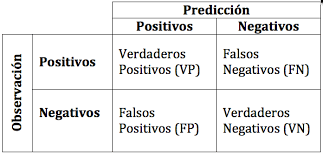
\includegraphics[width=2.5in]{images/confusion_matrix}
\end{center}
\caption{Matríz de Confusión}
\end{figure}

La estrategia solo toma la señal cuando el modelo predice un incremento en el precio, la venta por el contrario no depende del modelo, sino de los parámetros predefinidos (porcentaje de Stop Loss y Horizonte de tiempo). Esta característica implica que el valor a maximizar es la predicción de los verdaderos positivos, conocido como $Precisión$.

$$ Precisión = \frac{VP}{VP + FN} $$

\section{Bases Legales}


% !TeX root = ./main.Rnw
%\SweaveUTF8

\chapter{Marco Metódico}
\section{Análisis Exploratorio de los datos}

\subsection{Datos OHLC y Fuente de los datos}

La estructura de los datos utilizados en el trabajo es de tipo OHLC por sus siglas en inglés Open, High, Low, Close. La misma, resume en 4 registros el comportamiento del precio del activo (Apertura, Cierre, Mínimo y Máximo) en un intervalo de tiempo. En el caso de la presente investigación, de un día. Este tipo de dato provee la información necesaria para cubrir las exigencia del modelo, tanto para la creación de la variable dependiente como para el cálculo de los indicadores técnicos. 

Los datos fueron extraídos del portal www.investing.com, uno de los portales financieros con mayor prestigio en el mundo. Fue fundado en 2007 y es conocido por su prestigioso calendario económico y directorio de brokers.

\subsection{Series de Índices}

El universo de estudio está representado por los índices bursátiles de los mercados financieros existentes entre el período 26/10/2008 - 18/01/2019. Un índice búrsatil es un promedio de los precios de los activos que representan un mercado o sector determinado. Los mismos sirven como 'benchmark' o referencia de la economía de un país, sector financiero, etc. En el ámbito de los 'hedge funds' son una referencia para medir la rentabilidad de una estrategia de inversión y el riesgo del mercado.

En la presente investigación se utilizan los índices como reflejo del comportamiento de varios activos, de esta manera, se mide la estrategia en un sector y no en un instrumeto en específico. Otras de las ventajas de utilizar los índices es que al representar un promedio de varios activos, sus variaciones son menos drásticas. La muestra está constituida por 5 índices bursátiles que representan distintos mercados del mundo: NASDAQ, NIKKEI, FTSE 100, BOVESPA y SP500.

% hablar de cada indice


\begin{figure}[H]
\setkeys{Gin}{width =0.8\textwidth}
\centering
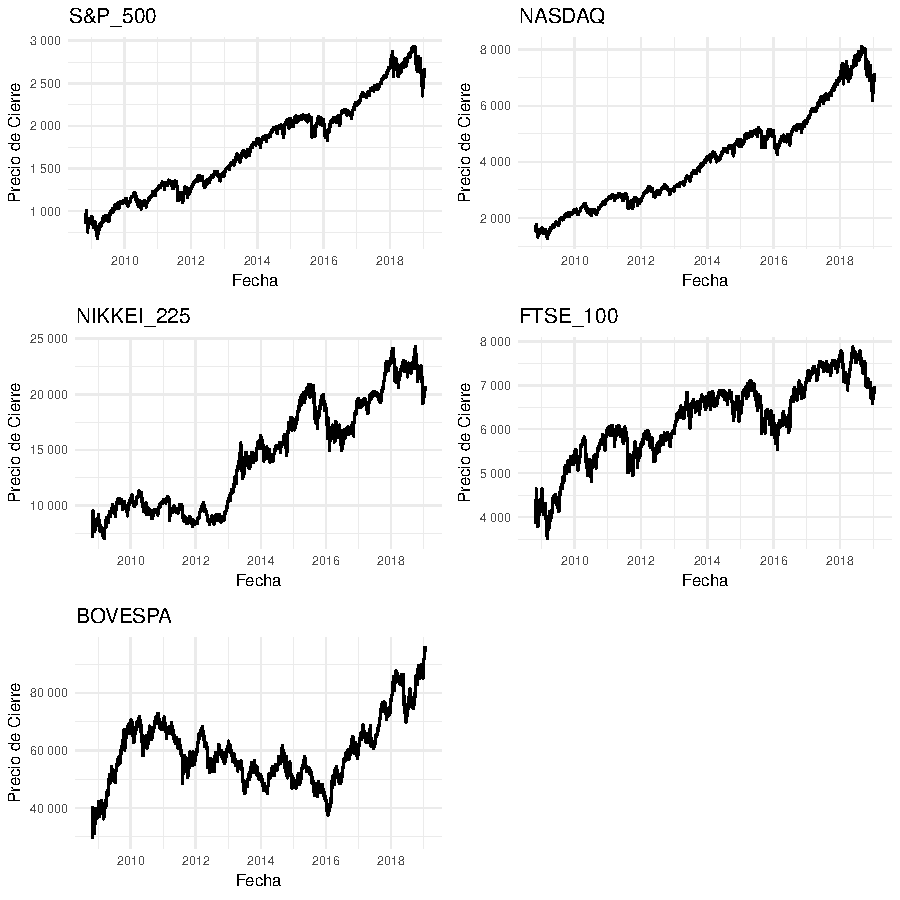
\includegraphics{main-002}
\caption{Precios de Cierre de los índices en el período de estudio (26/10/2008 - 18/01/2019)}
\end{figure}

\section{Entrenamiento del Modelo}

\subsection{Indicadores Técnicos como variables predictoras}

Los indicadores a utilizar fueron seleccionados buscando recoger la mayor información posible sobre el precio del activo que se pueden resumir en tres categorías: tendencia, momentum y volatilidad.

No es de interés en la presente investigación describir como funciona cada indicador para la toma de decisiones en el trading basado en fundamentos técnicos. Cada indicador puede utilizarse de distintas maneras, calcularse con distintos parámetros y asociarse a discreción del trader, lo que conlleva a un sin fin de reglas de asciación. 

Lo que busca la investigación es utilizar la relación entre estos indicadores como variables independientes que ayuden al modelo a predecir oportunidades de entradas. En este sentido se asume la existencia de una dinámica local del mercado que puede ser predecida con ayuda de estos indicadores.

Ahora bien, la idea base de la investigación era utilizar los valores de cada indicador en el análisis de componentes principales. Dado que el cálculo de todos los indicadores provienen de la misma variable -precio de cierre-, exite una alta colinealidad entre ellos, la idea de utilizar el ACP es precisamente para enfrentar este problema como se detallará mas adelante. Sin embargo, es de notar que los valores de los indicadores por sí solos no proveen un poder predictivo, lo que verdaderamente usa el trader son las asociaciones entre indicadores para encontrar patrones. 

Para enfrentar esta situación se decidió utilizar como predictores no los indicadores por si solos, sino, las relaciones entre cada uno de ellos. Esto se abordo agregando al modelo las interacciones entre todos indicador, y removiendo los indicadores por si solos. De esta manera el hecho de utilizar ACP, no solo es visto ahora como una manera de remover la colinealidad entre predictores sino como método de reducción de variables, ya que se paso de tener 19 predictores a 171.

A continuación se presentan una serie de graficos para regflejar lo anteriormente expuesto en relación a la colinealidad entre los indicadores

\subsection{Variable dependiente}

Las decisiones de entrada en el trading pueden ser producto de muchos factores, en la presente investigación se analiza el enfoque donde se define un porcentaje objetivo de ganancia y se intenta predecir si dicho objetivo se materializará en un futuro cercano, sin que se haya concretado una venta por Stop Loss. Este enfoque reduce la toma de decisión en una variable tal que:

$$
P_{X}(x) = 
\begin{array}{ll} 
\ \ \ \ p \ ; \qquad x = c
\\
\ 1-p \ ; \qquad x = -d
\end{array}
$$

Dado los datos OHLC del activo es posible identificar los períodos en donde se materializa la variable dependiente. la identificación se realiza, comparando el precio de cierre con los precios máximos y mínimos de las siguientes h observaciones, donde h es el número de períodos, en este caso días en los cuales se desea evaluar la condición.

En la práctica se identifica los registros que cumplen con esta condición añadiendo una columna a la data donde incluimos 'buy' para identificar los registros donde se da la señal y 'stay' en caso de que no haya ocurrido o hubiese ocurrido primero el retroceso del precio.

\subsection{Validación Cruzada en Series de Tiempo}

La validación Cruzada es un metódo de validación y prueba que consiste en dividir los registros aleatoriamente en grupos de similar tamaño. El primer grupo es utilizado como validación del modelo que ha sido entrenado en el resto de los datos, este proceso se realiza k veces, y el resultado final es el promedio arrojado por cada una de las k validaciones.

Ahora bien este método asume que no existe relación entre las observaciones, es decir que son independientes. Esto no es verdad en el caso de las series de tiempo debido a la condicion de autoregresión. Por lo tanto al dividir la data se debe respetar el orden temporal de cada observación. 

\subsection{WalkForward Backtesting}

Al principio de la investigación se implementó el método de entrenamiento, validación y prueba comúnmente utilizado, en donde la mayor parte de la data es destinada a entrenamiento del modelo, otra seccion es destinada a validación, para elegir los parámetros óptimos, y finalmente se testeaba el modelo en la data de prueba. Sin embargo este tipo de metodología en opinión del investigador no es el más óptimo para desarrollar el presente modelo, dado el dinamísmo de los mercados bursátiles la estrategia no puede permanecer estática en el tiempo.

Para contrarestar esta situación se opto por el método de $backtesting Walkforward$, el cual consiste en entrenar el modelo en un período base de data, en este caso los primeros 4 años de estudio, posteriormente se aplica la estrategia en el año siguiente y se obtiene los primeros resultados. Luego este año de aplicación es incluído en la data de entrenamiento -es decir, la data de entrenamiento pasa a ser de 5 años- y se evalúa el modelo en el siguiente año. De esta manera, contemplamos el dinamísmo del mercado permitiendole al modelo -y por ende a la estrategia- utilizar el período mas reciente con respecto al cual será implementado. En la presente figura se ilustra la metodología implementada.

\begin{figure}[ht]
\begin{center}
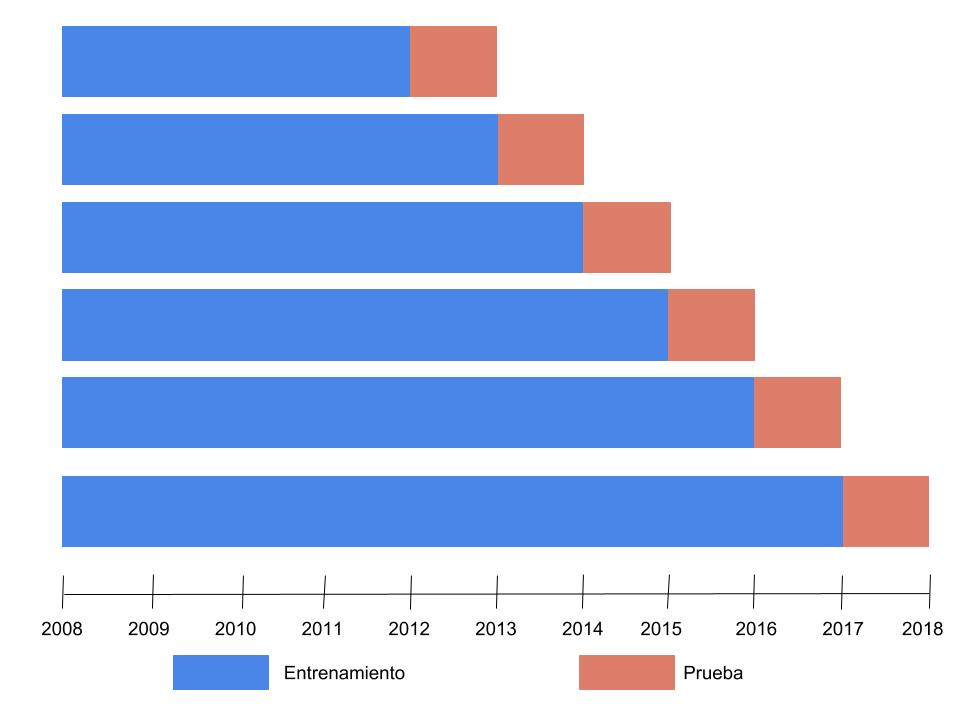
\includegraphics[width=2.5in]{images/walkforward_plot}
\end{center}
\caption{Metodología WalkForward}
\end{figure}

Otra de las caracteristicas de la metodología que se modificó fue la elección de los parámetros óptimos. Previamente se utilizaba la data de validación para buscar la combinación de parámetros óptima. Ahora bien en la metodología de Walkforward se utilizan los mismo parámetros. A opinión del investigador al buscar los mejores parámetros se estaría incurriendo en un posible cesgo de sobreoptimización. El hecho de que en un año determinado unas configuraciones óptimas den los mejores resultados no asegura que se replique en el siguiente año.

La selección de los parámetros debería ser un estudio previo de la serie financiera a testear. Evidentemente al seleccionar un período de tiempo mas corto se obtendrán menos observaciones que cumplan con el patrón por lo tanto se estaría en presencia de un problema de data imbalanceada que debe tener un tratamiento distinto. Por otro lado el utilizar un horizonte mayor no representa gran cambio en el número de ocurrencias, pero sí en el caso de que la transacción quede abierta -hay recordar que h representa una condición de salida para la estrategia de no ocurrir el target ni el stop loss-. La estrategia implementada en la invstigación toma un horizonte de 20 períodos ya que este valor representa un umbral para la ocurrencia del objetivo.


\begin{figure}[H]
\setkeys{Gin}{width =0.8\textwidth}
\centering
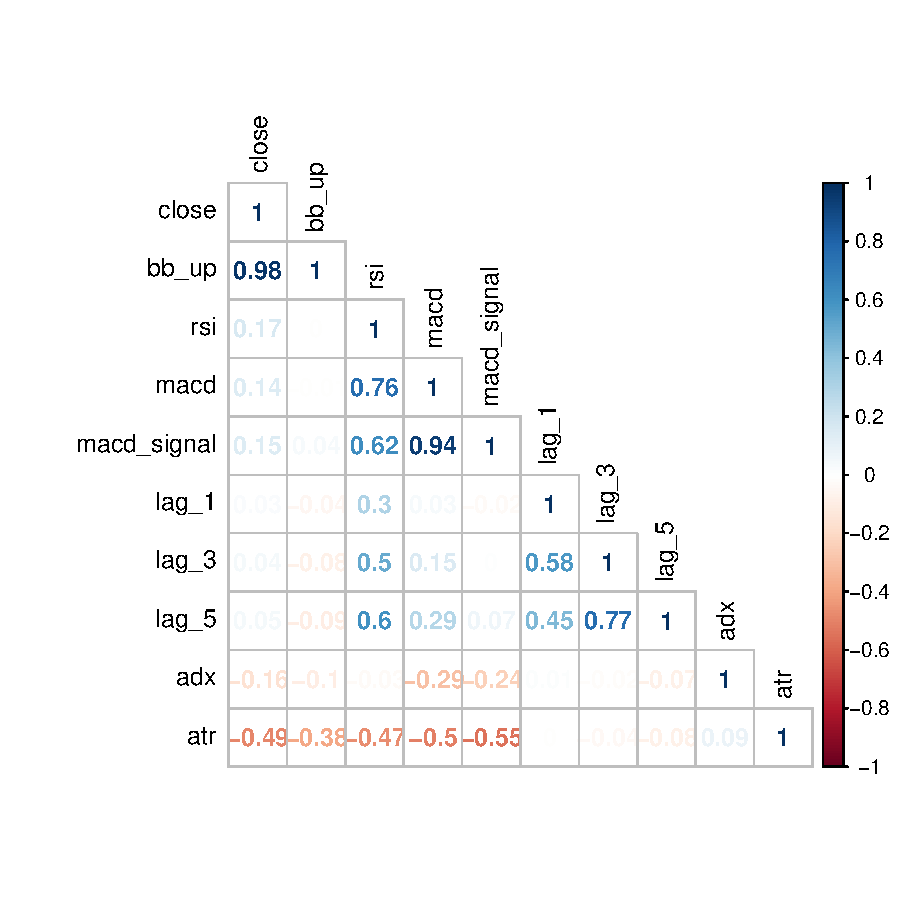
\includegraphics{main-004}
\caption{Observaciones que presentan ocurrencias con sl = 2.5\%, en el primer conjunto de datos de entrenamiento (26/10/2008 - 31/12/2010) para el índice S&P500, para diferentes valores de tp y h}
\end{figure}

\subsection{Reducción de la dimensión con Análisis de Componentes Principales}





% !TeX root = ./main.Rnw
%\SweaveUTF8

\chapter{Análisis de Resultados}

En el presente capítulo se realiza la descripción de los resultados obtenidos despues de la aplicación del método propuesto para la estrategia. De igual modo, se presentan los resultados arrojados por las pruebas de Backtesting simulando las entradas y salidas.

\section{Series de Rendimientos}



\begin{Schunk}
\begin{Sinput}
> 
\end{Sinput}
\end{Schunk}




% !TeX root = ./main.Rnw
%\SweaveUTF8

\chapter*{Conclusiones y Recomendaciones}
\addcontentsline{toc}{chapter}{Conclusiones y Recomendaciones}

El estudio presentado se centró en confirmar alternativas eficaces para el cálculo del VaR en mercados de materias primas. Los hechos estilizados de las series de tiempo financieras fueron considerados a los largo del trabajo. Y frente a estos planteamientos, se desarrolló una investigación que permitiera detectar una aproximación con el método GARCH-EVT-COPULAS que tuviese la capacidad de estimar el riesgo del mercado de commodities.\\

% !TeX root = ./main.Rnw
%\SweaveUTF8

\chapter*{Lista de Referencias}
\addcontentsline{toc}{chapter}{Lista de Referencias}

\begin{itemize}

\item Alexander, N. Y Zafer, D. (2016). \textit{Gestión del riesgo con el uso de commodities energéticos utilizando Valor en riesgo y Teoría del Valor Extremo}. Suecia, Universidad de Lund.

\end{itemize}

\end{document}
